% Basic document class
\documentclass[landscape, twocolumn, 12pt]{article}

% General public packages loaded here:
\usepackage{amsmath}
\usepackage{amssymb}
\usepackage{graphicx}
\usepackage{caption}
\usepackage{float}
\usepackage{pdfpages}
\usepackage{gensymb}
\usepackage{tikz}

% Custom .sty files loaded here:
\usepackage{TitlePage}
\usepackage{mathshortcuts}

% Add to glossary
% Check mathshortcuts.sty for documentation
\glo{Mu}{M_{u}}{Factored ultimate moment in the beam}
\glo{Mn}{M_n}{Nominal moment strength}
\glo{As}{A_s}{Area of tension reinforcing steel}
\glo{bb}{b}{Width of compression zone in a beam}
\glo{dd}{d}{Distance from the extreme fiber in compression}

\glo{rhob}{\rho_b}{The reinforcement ratio of concrete at the balance condition}

\glo{fy}{f_y}{Yield stress of steel}
\glo{fs}{f_s}{Stress of the steel}
\glo{fc}{f'_c}{Yield stress of concrete}
\glo{betao}{\beta_1}{ACI variable}

\glo{ecu}{\varepsilon_{cu}}{Ultimate compressive strain of concrete}
\glo{ey}{\varepsilon_y}{Yield strain of steel}
\glo{es}{\varepsilon_s}{Strain of tension steel}

% Title Page commands
% Check TitlePage.sty for documentation

\title{Concrete Beam Design}
\subtitle{Beam Design}
\coursenum{CEE421}
\coursetitle{Concrete Structures}
\university{Arizona State University}

\titleimage{Figures/Title.png}
\author{Brian Badahdah}
\date{\today}

%-------------------------------------------
\begin{document}

\maketitle


\section{Beam Analysis}
\subsection{The Whitney Stress Block}

The parameter \betao is calculated by equation \ref{Eq:betao} which is taken from ACI Table 22.2.2.4.3, where \fc  is taken to be in units of psi.

\begin{align}
	\betao
	=s
	\begin{cases}
		0.85 & \fc \leq 4000 \\
		0.85-0.05\left[\frac{\fc-4000}{1000}\right] & 4000 \leq\fc\leq 8000 \\
		0.65 & \fc > 8000
	\end{cases}
	\label{Eq:betao}
\end{align}



\subsection{The Balance Condition}

The balance condition is the condition which the concrete crushes at the same time that the steel yields. To solve for the neutral axis at the balance condition we use similar triangles.

\begin{align}
	\frac{c}{\ecu} &= \frac{d-c}{\es}\\ 
	c \es &= \ecu(d-c)\\ 
	c \es &= d\ecu -c\ecu\\ 
	c_{bal} &= \frac{d\ecu}{\es+\ecu}
\end{align}


Using $c_{bal}$ we can calculate the area of the steel \As at the balance condition.

\begin{align}
	\As &= \frac{0.85\fc\betao c_{bal}\bb}{\fy}
\end{align}

Next, we find the reinforcement ratio of the balance condition:

\begin{align}
	\rho_{bal} &= \frac{0.85\fc\betao}{\fy}
	\left[
		\frac{\ecu}{\es+\ecu}
	\right]\\
	&= 
	\frac{0.85\fc\betao}{\fy}
	\left[
		\frac{87}{87+\fy}
	\right]
\end{align}




\section{Beam Design}
\subsection{Deriving the Design Equations}

\begin{figure}[h]
\begin{tikzpicture}
	%% Cross section
	\draw[ultra thick] (1.5,3) rectangle (0,0);
	
	%% height
	\draw[thick,|<->|] (-0.5,0) -- node[left]{h} (-0.5,3);
	
	%% base
	\draw[thick,|<->|] (0,3.5) -- node[above]{\bb} (1.5,3.5);
	
	%% depth to steel
	\draw[thick,|<->|] (2,0.5) -- node[right]{\dd} (2,3);
	
	\draw[dashed, thin] (0,0.5) -- (10,0.5);
	
	\draw[dashed, thin] (-1,0) -- (10,0);
	\draw[dashed, thin] (-1,3) -- (10,3);
	
	%Steel circles
	\draw[ultra thick,fill=white] (0.5,0.5) circle (0.1cm);
	\draw[ultra thick,fill=white] (1,0.5) circle (0.1cm);
	
	%% Strain axis line
	\draw[ultra thick] (4,0) -- (4,3);
	% strain plot and labels
	\draw[thick,|<->|] (2.9,-0.5) -- node[below]{\es$\geq$\ey} (4,-0.5);
	\draw[dashed, thin] (2.9,-0.5) -- (2.9,0.5);
	
	\draw[thick] (2.5,0) -- (5,3);
	\draw[thick,|<->|] (5,3.5) -- node[above]{\ecu} (4,3.5);
	%Neutral axis
	\draw[thin, dashed] (3,1.8) -- (10, 1.8);
	% Depth to neutral axis line
	\draw[thick, |<->|] (3,1.8) -- node[left]{c} (3,3);
	
	\begin{scope}[xshift=-0.5cm]
	%% Stress axis line
	\draw[ultra thick] (7,0) -- (7,3);
	\draw[thick,|<->|] (6,2) -- node[left]{a} (6,3);
	\draw[thin, dashed] (6,2) -- (10,2);
	
	\draw[thick,|<->|] (7,3.5) -- node[above]{0.85\fc} (8,3.5);
	\draw[thick,|<->|] (6,-0.5) -- node[below]{\fs=\fy} (7,-0.5);
	
	%whitney stress block arrows
	\draw[thick,red,->] (8,3) -- (7,3);
	\draw[thick,red,->] (8,2.5) -- (7,2.5);
	\draw[thick,red,->] (8,2) -- (7,2);
	\draw[thick, red] (8,3) -- (8,2);
	
	% Steel stress
	\draw[thick, red, <-] (7,0.6) -- (5.5,0.6);
	\draw[thick, red, <-] (7,0.4) -- (5.5,0.4);
	\draw[thick, red] (5.5,0.4) -- (5.5,0.6);
	\end{scope}
	
	\begin{scope}[xshift=-0.5cm]
	%% Force axis line
	\draw[ultra thick] (9,0) -- (9,3);
	
	% Resultant forces
	% Comression
	\draw[ultra thick, red, <-] (9,2.5) -- node[above,fill=white]{$C_c$} (10,2.5);
	\draw[thick, |<->|] (10,2.5) -- node[right]{$\frac{a}{2}$} (10,3);
	%Tension
	\draw[ultra thick, red, ->] (8,0.5) -- node[below,fill=white]{$T_s$} (9,0.5);
	
	\draw[thick, |<->|] (10,2.5) -- node[fill=white]{$\dd-\frac{a}{2}$} (10,0.5);
	
	\end{scope}
	
\end{tikzpicture}
\end{figure}

Equation \ref{Eq:design} is the basic design relationship for concrete beams.


\begin{align}
	\phi \Mn \geq \Mu
	\label{Eq:design}
\end{align}

where \Mn is the nominal moment in the beam and \Mu is the ultimate moment in the beam.

The nominal moment of the beam is found by taking moments about the resultant compressive force. The only force left is the tension force in the steel.

\begin{align}
	\phi T_s z \geq \Mu
\end{align}

Next, plug in the force in the tension steel and the distance from the compressive force to the tensile force. Note that the force in the tension steel is taken to be the area of the steel multiplied by the yield stress. This is because the steel is assumed to be yielding.

\begin{align}
	\phi
	\left(\As \fy\right)
	\left(d-\frac{1}{2}a\right)
	\geq
	\Mu
	\label{Eq:2}
\end{align}

Now we will derive the height of the ``Whitney Stress block'' or the ``equivalent stress block''. From equilibrium we know the tensile force in the steel will be equal to the compressive force in the concrete. This fact will be used to isolate the height of the stress block

\begin{align}
	T_s &= C_c\\
	\As \fy &= 0.85 \fc ab
\end{align}

Solve for $a$

\begin{align}
	a&=\frac{\As \fy}{0.85f'_cb}
\end{align}


Next, plug in the value of $a$ into equation \ref{Eq:2}.

\begin{align}
	\phi
	\left(\As \fy\right)
	\left(d-\frac{1}{2}\frac{\As \fy}{0.85f'_cb}\right)
	\geq
	\Mu
\end{align}

We want to get the equation in terms of the \textit{reinforcement ratio}, $\rho$. We can accomplish this by dividing both sides of the equation by $bd^2$.


\begin{align}
	\phi
	\left(\frac{\As}{bd} \fy\right)
	\left(\frac{d}{d} - \frac12\frac{\As\fy}{0.85\fc bd}\right)
	\geq
	\frac{\Mu}{bd^2}
\end{align}


Substitute the reinforcement ratio into the equation

\begin{align}
	\phi
	\left(\rho \fy\right)
	\left(1 - \frac12\frac{\rho \fy}{0.85 \fc}\right)
	\geq
	\Mu
\end{align}



To calculate the reinforcement ratio at the balance condition:

\begin{align}
	c_{bal} =
	\left[
		\frac{\ecu}{\ecu + \ey}
	\right]
	\dd
\end{align}


\begin{align}
	\rho_{bal} = 
	\frac{0.85\fc\betao}{\fy}
	\left[
		\frac{87}{\fy+87}
	\right]
\end{align}



\begin{align}
	\rho_{design}=\frac{0.75\rhob}{2}
\end{align}


\begin{align}
	\phi R \geq \frac{\Mu}{bd^2}
	\label{Eq:design2}
\end{align}

where

\begin{align}
	R(\fc,\fy,\rho) = 
	\rho \fy 
	\left(1-\frac{\fy}{1.7\fc \rho}\right)
\end{align}



To solve for the depth of the neutral axis:

\begin{align}
	T &= C\\
	\As\fs &=0.85\fc a b\\ 
	\As E_s \es &= 0.85\fc \betao c b\\
	\As E_s \frac{\ecu(d-c)}{c} &= 0.85\fc \betao c b\\
	\As E_s (d-c) \ecu &= 0.85 \fc \betao c^2 b\\ 
\end{align}

Solving for the neutral axis $c$ is a matter of using the quadratic formula. This requires putting the equation into the following form:

\begin{align}
		0.85 \fc \betao c^2 b + \As E_s \ecu c - \As E_s \ecu d &= 0
		\label{Eq:neutralaxis}
\end{align}


Table \ref{Tab:bars} shows the dimensions of reinforcing steel bars.

\begin{table}[h]
\centering
\caption{Areas, Weights, and Dimensions of Reinforcing Bars}
\label{Tab:bars}
\begin{tabular}{|c|c|c|c|}\hline
Bar Size (No.)&Weight (lb/ft)&Diameter(in.)&Area (in.$^2$) \\ \hline
3&0.376&0.375&0.11 \\ \hline
4&0.668&0.500&0.20 \\ \hline
5&1.043&0.625&0.31 \\ \hline
6&1.502&0.750&0.44 \\ \hline
7&2.044&0.875&0.60 \\ \hline
8&2.67&1.000&0.79 \\ \hline
9&3.40&1.128&1.00 \\ \hline
10&4.30&1.270&1.27 \\ \hline
11&5.31&1.410&1.56 \\ \hline
14&7.65&1.693&2.25 \\ \hline
18&13.60&2.257&4.00 \\ \hline
\end{tabular}
\end{table}



\subsection{Automating beam design}


Taking the fundamental design equation from equation \ref{Eq:design2} and rearranging for the $bd^2$ term yields:

\begin{align}
	bd^2=\frac{\Mu}{\phi R(\fc,\fy,\rho)}
\end{align}

Now, we can take this equation and divide both sides $d^3$. This puts the left side as the ratio of $b/d$ and the right side is only dependent on $d^3$.

\begin{align}
	\frac{b}{d}=\frac{\Mu}{d^3 \phi R(\fc,\fy,\rho)}
\end{align}

The ideal ratio is between 0.4 and 0.6. This can be substituted on the left side of the equation as a constant value which can be specified as an input. Furthermore the equation is rewritten such that all terms are on the right side and the equation is equal to zero.


\gbox{
	g(d)=\frac{\Mu}{d^3 \phi R(\fc,\fy,\rho)}-\lambda_1
	\label{Eq:Residual}
}

The tangent to this residual equation is:

\gbox{
	A(d) = -\frac{3}{d^4}\frac{\Mu}{\phi R(\fc, \fy, \rho)}
	\label{Eq:Tangent}
}

The root of the residual equation can be solved using Newton's method.


\begin{pseudocode}
 \item Input physical quantities (\fc,\fy,etc...)
 \item Define relevant functions
 \item Set-up and execute Newton's method to solve for $d$
 \begin{enumerate}
 	\item Use the residual $g(d)$ and tangent $A(d)$ from equations \ref{Eq:Residual} and \ref{Eq:Tangent}, respectively.
 	\item Calculate $b$ given the value of $d$ once the solution has converged
 \end{enumerate}
 
 \item Round up values of $b$ and $d$
	\item Loop through possible bar sizes in table \ref{Tab:bars}
	\begin{enumerate}
		\item Calcualte number of bars required for each size
		\item Calculate the width required for that bar No.
		\item If it meets the spacing requirements add it to a list of usable candidates
	\end{enumerate}

 \item Compute neutral axis from equation \ref{Eq:neutralaxis}
 \item Check that the steel is yielding
\end{pseudocode}

\section{Beam Design}
\subsection{Deriving the Design Equations}

\begin{figure}[h]
\begin{greenfig}
\begin{tikzpicture}[xscale=0.95]
	%% Cross section
	\draw[ultra thick] (1.5,3) rectangle (0,0);

	%% height
	\draw[thick,|<->|] (-0.5,0) -- node[left]{h} (-0.5,3);

	%% base
	\draw[thick,|<->|] (0,3.5) -- node[above]{\bb} (1.5,3.5);

	%% depth to steel
	\draw[thick,|<->|] (2,0.5) -- node[right]{\dd} (2,3);

	\draw[dashed, thin] (0,0.5) -- (10,0.5);

	\draw[dashed, thin] (-1,0) -- (10,0);
	\draw[dashed, thin] (-1,3) -- (10,3);

	%Steel circles
	\draw[ultra thick,fill=white] (0.5,0.5) circle (0.1cm);
	\draw[ultra thick,fill=white] (1,0.5) circle (0.1cm);

	%% Strain axis line
	\draw[ultra thick] (4,0) -- (4,3);
	% strain plot and labels
	\draw[thick,|<->|] (2.9,-0.5) -- node[below]{\es$\geq$\ey} (4,-0.5);
	\draw[dashed, thin] (2.9,-0.5) -- (2.9,0.5);

	\draw[thick] (2.5,0) -- (5,3);
	\draw[thick,|<->|] (5,3.5) -- node[above]{\ecu} (4,3.5);
	%Neutral axis
	\draw[thin, dashed] (3,1.8) -- (10, 1.8);
	% Depth to neutral axis line
	\draw[thick, |<->|] (3,1.8) -- node[left]{c} (3,3);

	\begin{scope}[xshift=-0.5cm]
	%% Stress axis line
	\draw[ultra thick] (7,0) -- (7,3);
	\draw[thick,|<->|] (6,2) -- node[left]{a} (6,3);
	\draw[thin, dashed] (6,2) -- (10,2);

	\draw[thick,|<->|] (7,3.5) -- node[above]{0.85\fc} (8,3.5);
	\draw[thick,|<->|] (6,-0.5) -- node[below]{\fs=\fy} (7,-0.5);

	%whitney stress block arrows
	\draw[thick,red,->] (8,3) -- (7,3);
	\draw[thick,red,->] (8,2.5) -- (7,2.5);
	\draw[thick,red,->] (8,2) -- (7,2);
	\draw[thick, red] (8,3) -- (8,2);

	% Steel stress
	\draw[thick, red, <-] (7,0.6) -- (5.5,0.6);
	\draw[thick, red, <-] (7,0.4) -- (5.5,0.4);
	\draw[thick, red] (5.5,0.4) -- (5.5,0.6);
	\end{scope}

	\begin{scope}[xshift=-0.5cm]
	%% Force axis line
	\draw[ultra thick] (9,0) -- (9,3);

	% Resultant forces
	% Comression
	\draw[ultra thick, red, <-] (9,2.5) -- node[above,fill=mattegreen]{$C_c$} (10,2.5);
	\draw[thick, |<->|] (10,2.5) -- node[right]{$\frac{a}{2}$} (10,3);
	%Tension
	\draw[ultra thick, red, ->] (8,0.5) -- node[below,fill=mattegreen]{$T_s$} (9,0.5);

	\draw[thick, |<->|] (10,2.5) -- node[fill=mattegreen]{$\dd-\frac{a}{2}$} (10,0.5);

	\end{scope}

\end{tikzpicture}
\end{greenfig}
\end{figure}

Equation \ref{Eq:design} is the basic design relationship for concrete beams.


\begin{align}
	\phi \Mn \geq \Mu
	\label{Eq:design}
\end{align}

where \Mn is the nominal moment capacity of the beam and \Mu is the ultimate moment in the beam.

The nominal moment of the beam is found by taking moments about the resultant compressive force. The only force left is the tension force in the steel.

\begin{align}
	\phi T_s z \geq \Mu
\end{align}

Next, plug in the force in the tension steel and the distance from the compressive force to the tensile force. Note that the force in the tension steel is taken to be the area of the steel multiplied by the yield stress. This is because the steel is assumed to be yielding.

\begin{align}
	\phi
	\left(\As \fy\right)
	\left(d-\frac{1}{2}a\right)
	\geq
	\Mu
	\label{Eq:2}
\end{align}

Now we will derive the height of the ``Whitney Stress block'' or the ``equivalent stress block''. From equilibrium we know the tensile force in the steel will be equal to the compressive force in the concrete. This fact will be used to isolate the height of the stress block

\begin{align}
	T_s &= C_c\\
	\As \fy &= 0.85 \fc ab
\end{align}

Solve for $a$

\begin{align}
	a&=\frac{\As \fy}{0.85f'_cb}
\end{align}


Next, plug in the value of $a$ into equation \ref{Eq:2}.

\begin{align}
	\phi
	\left(\As \fy\right)
	\left(d-\frac{1}{2}\frac{\As \fy}{0.85f'_cb}\right)
	\geq
	\Mu
\end{align}

We want to get the equation in terms of the \textit{reinforcement ratio}, $\rho$. We can accomplish this by dividing both sides of the equation by $bd^2$.


\begin{align}
	\phi
	\left(\frac{\As}{bd} \fy\right)
	\left(\frac{d}{d} - \frac12\frac{\As\fy}{0.85\fc bd}\right)
	\geq
	\frac{\Mu}{bd^2}
\end{align}


Substitute the reinforcement ratio into the equation

\begin{align}
	\phi
	\left(\rho \fy\right)
	\left(1 - \frac12\frac{\rho \fy}{0.85 \fc}\right)
	\geq
	\Mu
\end{align}


\begin{align}
	\rho_{design}=\frac{0.75\rhob}{2}
\end{align}


\begin{align}
	\phi R \geq \frac{\Mu}{bd^2}
	\label{Eq:design2}
\end{align}

where

\begin{align}
	R(\fc,\fy,\rho) =
	\rho \fy
	\left(1-\frac{\rho\fy}{1.7\fc}\right)
\end{align}



To solve for the depth of the neutral axis:

\begin{align}
	T &= C\\
	\As\fs &=0.85\fc a b\\
	\As E_s \es &= 0.85\fc \betao c b\\
	\As E_s \frac{\ecu(d-c)}{c} &= 0.85\fc \betao c b\\
	\As E_s (d-c) \ecu &= 0.85 \fc \betao c^2 b
\end{align}

Solving for the neutral axis $c$ is a matter of using the quadratic formula. This requires putting the equation into the following form:

\gbox{
		0.85 \fc \betao c^2 b + \As E_s \ecu c - \As E_s \ecu d &= 0
		\label{Eq:neutralaxis}
}

\subsection{Spacing Requirements}
When designing beams you must ensure that there is enough horizontal space to fit the steel bars. The width of the beam must fit the diameters of the bars, ACI required spacing between the bars, and cover on the left and right of the bars. The minimum spacing between bars is the maximum of the following three items as per ACI 25.2.1.

\begin{itemize}
	\item 1 inch
	\item $\frac{4}{3}$ diameter of largest aggregate
	\item diameter of the reinforcing bar
\end{itemize}



\subsection{Automating beam design}


Taking the fundamental design equation from equation \ref{Eq:design2} and rearranging for the $bd^2$ term yields:

\begin{align}
	bd^2=\frac{\Mu}{\phi R(\fc,\fy,\rho)}
\end{align}

Now, we can take this equation and divide both sides $d^3$. This puts the left side as the ratio of $b/d$ and the right side is only dependent on $d^3$.

\begin{align}
	\frac{b}{d}=\frac{\Mu}{d^3 \phi R(\fc,\fy,\rho)}
\end{align}

The ideal ratio is between 0.4 and 0.6. This can be substituted on the left side of the equation as a constant value which can be specified as an input. Furthermore the equation is rewritten such that all terms are on the right side and the equation is equal to zero.


\gbox{
	g(d)=\frac{\Mu}{d^3 \phi R(\fc,\fy,\rho)}-\lambda_1
	\label{Eq:Residual}
}

The tangent to this residual equation is:

\gbox{
	A(d) = -\frac{3}{d^4}\frac{\Mu}{\phi R(\fc, \fy, \rho)}
	\label{Eq:Tangent}
}

The root of the residual equation can be solved using Newton's method.

\gbox{
	\dd_{i+1} = \dd_i - \frac{g(\dd_i)}{A(\dd_i)}
}

\vfill
\begin{pseudocode}
	\item Input physical quantities (\fc, \fy, etc...)
	\item Define relevant functions
	\item Set-up and execute Newton's method to solve for $d$

	\begin{enumerate}
	\item Use the residual $g(d)$ and tangent $A(d)$ from equations \ref{Eq:Residual} and \ref{Eq:Tangent}, respectively.
	\item Calculate $b$ given the value of $d$ once the solution has converged
	\end{enumerate}

	\item Round up values of \bb and \dd
	\item Calculate the neeeded \As   from $\rho_{design}$

	\item Loop through possible bar sizes in table \ref{Tab:bars}

	\begin{enumerate}
		\item Calcualte number of bars required for each size
		\item Calculate the width required for that bar No.
		\item If it meets the spacing requirements add it to a list of usable candidates
	\end{enumerate}

	\item Compute neutral axis from equation \ref{Eq:neutralaxis}
	\item Check that the steel is yielding
	\item Print and plot results
\end{pseudocode}
\hfill



\section{T-Beams}

\begin{figure}[h]
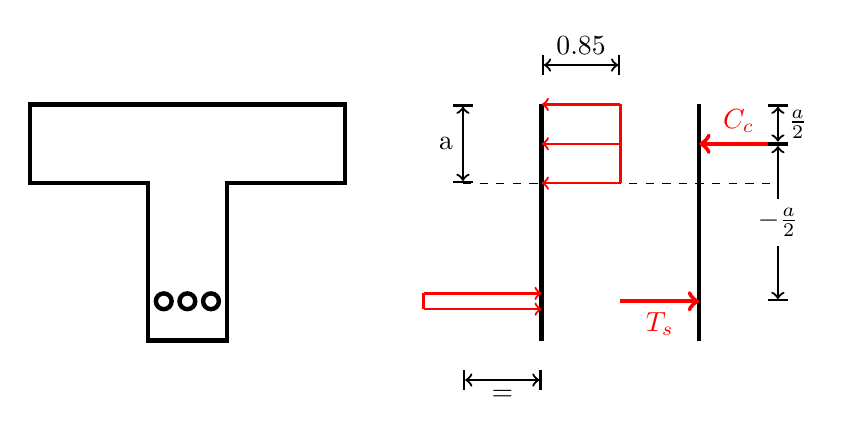
\begin{tikzpicture}
	
	
	\begin{scope}
	
	\pgfmathsetmacro{\be}{4}
	\pgfmathsetmacro{\H}{3}
	\pgfmathsetmacro{\hf}{1}
	
	\coordinate (A) at (0, \H);
	\coordinate (B) at (\be,\H);
	\coordinate (C) at (\be,\H-\hf);
	\coordinate (D) at (2.5,\H-\hf);
	\coordinate (E) at (2.5,0);
	\coordinate (F) at (1.5,0);
	\coordinate (G) at (1.5,2);
	\coordinate (H) at (0,2);
	
	\draw[ultra thick] 
		(A) -- 
		(B) -- 
		(C) --
		(D) -- 
		(E) -- 
		(F) -- 
		(G) -- 
		(H) --
		cycle;
	
	\draw[ultra thick,fill=white] (2,0.5) circle (0.1cm);
	\draw[ultra thick,fill=white] (2.3,0.5) circle (0.1cm);
	\draw[ultra thick,fill=white] (1.7,0.5) circle (0.1cm);
	\end{scope}
	

	
	\begin{scope}[xshift=-0.5cm]
	%% Stress axis line
	\draw[ultra thick] (7,0) -- (7,3);
	\draw[thick,|<->|] (6,2) -- node[left]{a} (6,3);
	\draw[thin, dashed] (6,2) -- (10,2);
	
	\draw[thick,|<->|] (7,3.5) -- node[above]{0.85\fc} (8,3.5);
	\draw[thick,|<->|] (6,-0.5) -- node[below]{\fs=\fy} (7,-0.5);
	
	%whitney stress block arrows
	\draw[thick,red,->] (8,3) -- (7,3);
	\draw[thick,red,->] (8,2.5) -- (7,2.5);
	\draw[thick,red,->] (8,2) -- (7,2);
	\draw[thick, red] (8,3) -- (8,2);
	
	% Steel stress
	\draw[thick, red, <-] (7,0.6) -- (5.5,0.6);
	\draw[thick, red, <-] (7,0.4) -- (5.5,0.4);
	\draw[thick, red] (5.5,0.4) -- (5.5,0.6);
	\end{scope}
	
	\begin{scope}[xshift=-0.5cm]
	%% Force axis line
	\draw[ultra thick] (9,0) -- (9,3);
	
	% Resultant forces
	% Comression
	\draw[ultra thick, red, <-] (9,2.5) -- node[above,fill=white]{$C_c$} (10,2.5);
	\draw[thick, |<->|] (10,2.5) -- node[right]{$\frac{a}{2}$} (10,3);
	%Tension
	\draw[ultra thick, red, ->] (8,0.5) -- node[below,fill=white]{$T_s$} (9,0.5);
	
	\draw[thick, |<->|] (10,2.5) -- node[fill=white]{$\dd-\frac{a}{2}$} (10,0.5);
	
	\end{scope}
	
\end{tikzpicture}
\end{figure}

%---------------------------------------------
\clearpage
\glsaddall
\printglossary[title={Variables Definitions}]
%\newpage
%\bibliography{References}
%\addcontentsline{toc}{section}{References}
%\bibliographystyle{apalike}
\end{document}